\documentclass[10pt]{article}

\usepackage{fullpage} % Package to use full page
\usepackage{parskip} % Package to tweak paragraph skipping
\usepackage{tikz} % Package for drawing
\usepackage{amsmath}
\usepackage{hyperref}
\usepackage{graphics,multirow,cases,algorithm,algpseudocode}
\usepackage{booktabs,color,comment}
\usepackage[english]{babel}
\usepackage{amsmath,amsthm,amssymb,verbatim,bbm}
%\usepackage[framed,numbered,autolinebreaks,useliterate]{mcode}
\usepackage{url}
\usepackage{nomencl}
\usepackage{enumitem}
\usepackage{siunitx}

\usepackage[normalem]{ulem}

\newcommand*{\bbar}[1]{\bar{\bar{#1}}}

\newcommand{\R}{{\mathcal{R}}}
\newcommand{\T}{{\mathcal{T}}}
\newcommand{\D}{{\mathcal{D}}}
\newcommand{\F}{{\mathcal{F}}}
\renewcommand{\S}{{\mathcal{S}}}
\newcommand{\spb}{{\smallskip}}
\newcommand{\mpb}{{\medskip}}
\newcommand{\bpb}{{\bigskip}}
\newcommand{\IN}{{\mathbb{N}}}
\newcommand{\IM}{{\mathbb{M}}}
\newcommand{\IZ}{{\mathbb{Z}}}
\newcommand{\IR}{{\mathbb{R}}}
\newcommand{\IE}{{\mathbb{E}}}
\newcommand{\IP}{{\mathbb{P}}}
\newcommand{\IC}{{\mathbb{C}}}
\newcommand{\mO}{{\mathcal{O}}}
%\newcommand{\IR}{{\mathbb{R}}}
%\newcommand{\IC}{{\mathbb{C}}}
%\newcommand{\IN}{{\mathbb{N}}}
%\newcommand{\IE}{{\mathbb{E}}}
%\newcommand{\IP}{{\mathbb{P}}}
\newcommand{\mF}{{\mathcal{F}}}
\newcommand{\mE}{{\mathcal{E}}}
\newcommand{\tT}{\intercal}
\newcommand{\mT}{{\mathcal{T}}}
\newcommand{\mconv}{{\mathrm{conv}}}
\newcommand{\mC}{{\mathcal{C}}_{2 \pi}}
\newcommand{\IX}{{\mathbb{X}}} %domain
\newcommand{\IS}{{\mathbb{S}}} %domain
\newcommand{\ID}{{\mathbb{D}}}
\newcommand{\IY}{{\mathbb{Y}}}
\newcommand{\cSm}{{\cal S}^{(m)}}
\newcommand{\cS}{{\cal S}_N}
\newcommand{\SM}{{\mathcal{P}}}
\newcommand{\SN}{{\mathcal{Q}}}
\newcommand{\SB}{{\mathcal{B}}}
\newcommand{\SD}{{\mathcal{D}}}

\newcommand{\iin}{\frac{i}{n}}
\newcommand{\jjn}{\frac{j}{n}}
\newcommand{\sumi}{\dsum_{i=1}^{n}}
\newcommand{\sumN}{\dsum_{i=1}^{N}}
\newcommand{\sumT}{\dsum_{t=1}^{T}}
\newcommand{\sumj}{\dsum_{j=1}^{n}}
\newcommand{\sumij}{\dsum_{i<j}}
\newcommand{\Xt}{{X_{t}}}
\newcommand{\Yt}{{Y_{t}}}
\newcommand{\la}{{\lambda}}
\newcommand{\bA}{{\bf A}}
\newcommand{\bB}{{\bf B}}
\newcommand{\bC}{{\bf C}}
\newcommand{\bAs}{{\bf A}_{\epsilon}}
\newcommand{\Bs}{B^{(\epsilon)}}
\newcommand{\bT}{{\bf T}}
\newcommand{\bu}{{\bf u}}
\newcommand{\bb}{{\bf b}}
\newcommand{\cT}{{\cal T}}
\newcommand{\cW}{{\cal W}}
\newcommand{\cC}{{\cal C}_{\epsilon}}
\newcommand{\cD}{{\mathcal{D}}}
\newcommand{\dx}{\Delta x}
\newcommand{\dt}{\Delta t}
\newcommand{\ep}{\epsilon}
\newcommand{\pC}{\partial C}

\makenomenclature
\renewcommand{\nomname}{List of Symbols}
%\renewcommand{\nompreamble}{The next list describes several symbols that will be later used within the body of the document}

\newenvironment{definition}[2][Definition]{\begin{trivlist}
\item[\hskip \labelsep {\bfseries #1}\hskip \labelsep {\bfseries #2.}]}{\end{trivlist}}
\newenvironment{theorem}[2][Theorem]{\begin{trivlist}
\item[\hskip \labelsep {\bfseries #1}\hskip \labelsep {\bfseries #2.}]}{\end{trivlist}}
\newenvironment{lemma}[2][Lemma]{\begin{trivlist}
\item[\hskip \labelsep {\bfseries #1}\hskip \labelsep {\bfseries #2.}]}{\end{trivlist}}
\newenvironment{exercise}[2][Exercise]{\begin{trivlist}
\item[\hskip \labelsep {\bfseries #1}\hskip \labelsep {\bfseries #2.}]}{\end{trivlist}}
\newenvironment{reflection}[2][Reflection]{\begin{trivlist}
\item[\hskip \labelsep {\bfseries #1}\hskip \labelsep {\bfseries #2.}]}{\end{trivlist}}
\newenvironment{proposition}[2][Proposition]{\begin{trivlist}
\item[\hskip \labelsep {\bfseries #1}\hskip \labelsep {\bfseries #2.}]}{\end{trivlist}}
\newenvironment{corollary}[2][Corollary]{\begin{trivlist}
\item[\hskip \labelsep {\bfseries #1}\hskip \labelsep {\bfseries #2.}]}{\end{trivlist}}

\DeclareMathOperator*{\argminA}{arg\,min} % Jan Hlavacek
\DeclareMathOperator*{\argminB}{argmin}   % Jan Hlavacek
\DeclareMathOperator*{\argminC}{\arg\min}   % rbp


% Latin text highlight
\def\latin#1{\emph{#1}}

% Mark-up commands
\def\Red#1{\textbf{\textcolor{red}{#1}}}	% for authors
\def\Blue#1{\textbf{\textcolor{blue}{#1}}}	% for reviewers


\title{TDA - filament network classification}
%\author{Le Yin, Ephy Love}
\date{November 2019}

% path to graphics
\graphicspath{{figures/}}

\begin{document}

\maketitle

\begin{abstract}

The actin cytoskeleton plays a critical role in plant cells. This filamentous structure of actin proteins can be viewed as a network. We show that key factors in the actin network generation process can be efficiently studied with network classification. We propose two novel, automated, classifiers, combining topological data analysis with a machine learning framework. One is a distance-based classifier in which a new distance on the persistence diagram space is adopted. The second is a non-distance-based classifier with a re-sampling process and persistence vectorization. Both classifiers are built on the persistent homology and persistence diagrams of simulated actin networks. We succeed in classifying these simulated networks with very high accuracy.

    \textbf{Keywords:} 
    
    \textbf{Running head:} 
\end{abstract}

\section{Introduction}
The actin cytoskeleton is a complex network of proteins that is present in all eukaryotic cells. In addition to its function as cellular scaffolding, the actin cytoskeleton enables several basic cellular functions including the control of cellular shape and direction of movement \cite{thomas2009actin}. These basic functions are critical to many higher order physiological processes such as cell division, expansion, mobility and motility\cite{freedman2017versatile}. 

In the actin cytoskeleton, actin filament organization is thought to be governed partially by the interaction of filaments and partially by myosin motor proteins. Actin filaments are polar structures, ploymerized by globular actin proteins. Many actin-binding proteins have potential to bind to actin filaments at various sites along the filament. These binding proteins allow actin filaments to assemble and disassemble spatiotemporally. The binding proteins give rise to a dense cross-linking where filaments develop into networks at with many filaments and binding sites. To understand certain behaviors of cells, it is of tremendous importance to understand the processes that govern actin filament network organization. A key driver of these processes may be the relationship between actin-binding proteins, individual filaments and emergent networks.

One method to study the actin filament network generating process is to simulate the dynamic structure of filament networks, combining theory from theoretical physical with experimental stochastic simulation. With this methodology one can control the known factors, which will affect the structure of networks. Varying these initial conditions enables researchers to compare the conditional difference in outcomes of the simulated networks. This experimental strategy can provide an opportunity to independently examine the role each factor plays in the process. These factors could include the cross-linker density(number of cross-linkers per certain area), cross-linker stiffness, maximum angle that can exist between two filament segments to be crosslinked, and so on\cite{freedman2017versatile,freedman2018nonequilibrium}. In this work, we propose a machine learning approach to classify filament networks generated with varied cross-linker density. Our method leverages the topology of the actin networks through Topological Data Analysis(TDA). Our exploratory work is the first time filament networks have been studied by classification. This work could serve as a pilot for future research in actin cytoskeleton organization. In the future, this work should be useful in the course of research on cytoplasmic streaming to be able to classify real cells based on images of their actin networks. This could provide biologists a method of disentangling the interaction of myosin motor proteins, the actin network, and streaming, i.e. by imaging the actin structure and clustering cells based on their actin network topology, the researcher may be able to fix a network structure while varying parameters specific to myosin.

In the fast developing field of machine learning, TDA has become increasingly popular as a powerful tool for classification. Researchers have used TDA to solve many real-world problems. Many TDA applications have been developed including signal identification \cite{marchese2016topological}, materials classification \cite{hiraoka2016hierarchical,maroulas2019bayesian}, shape recognition \cite{bonis2016persistence,li2014persistence}, histologic image analysis \cite{belchi2018lung,nicolau2011topology,singh2014topological}, ecology of human mobility \cite{chen2017measuring,chen2019generalized}, and cosmology \cite{sousbie2011persistent,van2010alpha}. A review of TDA and its application is provided in \cite{wasserman2018topological}. A sub-method of TDA, persistence homology, has been used to measure differences in topological features. Persistence homology records when homological features appear and vanish within data, and these patterns of persistence vary between samples. All of the appearances and disappearances of homological features are summarised in persistence diagrams. In this work, we encode the geometric features of filaments networks into persistence diagrams and classify simulated actin networks by calculating their similarities in a persistence space. We also show a method on the vectorization of the persistence space, as a persistence space is not itself a vector space.

The structure of this work is as follows: In section 2, we describe the data and introduce the background of persistence homology. Section 3 demonstrates two algorithms for classifying filament networks. Section 4 exhibits the numerical results. Section 5 will give conclusions and a discussion of future directions.


\section{Persistence Homology and Filament Networks}
As discussed, actin filaments are thought to be organized by cross-linking on actin-binding proteins. Filaments and inter-filament structure can then be simulated by a physical model \cite{freedman2017versatile,freedman2018nonequilibrium}. The change of initial conditions in a eukaryotic cell will cause variation in later measurement of filament networks. Our network data is simulated by three different cross-linker densities. Higher cross-linker density means more opportunities for filaments to be cross-linked, i.e. the binding and unbinding processes can be more active. As shown in Fig. \ref{fig:rawdata}(a), three kinds of filaments networks were simulated with different numbers of cross-linkers:  $825$, $1650$ and $3300$. All simulated cells were bound by a $\SI{20}{\micro\metre} \times \SI{20}{\micro\metre}$ square. Therefore, the cross-linker density of each network is $2.06$, $4.13$ and $8.25$ per $\SI{}{\micro\metre}^2$, respectively. In each network, there are a total of $100$ filaments with average length $\SI{10}{\micro\metre}$, where filaments are model as polar warm-like chain in red and blue dots represent barbed ends of these filaments. We also record the locations of the actin beads that make up the filaments, which are shown as small black circles in Fig. \ref{fig:rawdata}(b). Each actin bead is of radius $\SI{0.5}{\micro\metre}$. Our interest is in developing an automated method to accurately classify cross-linker density of filament networks from simulated network data.

\begin{figure}[tbp]
	\begin{center}
		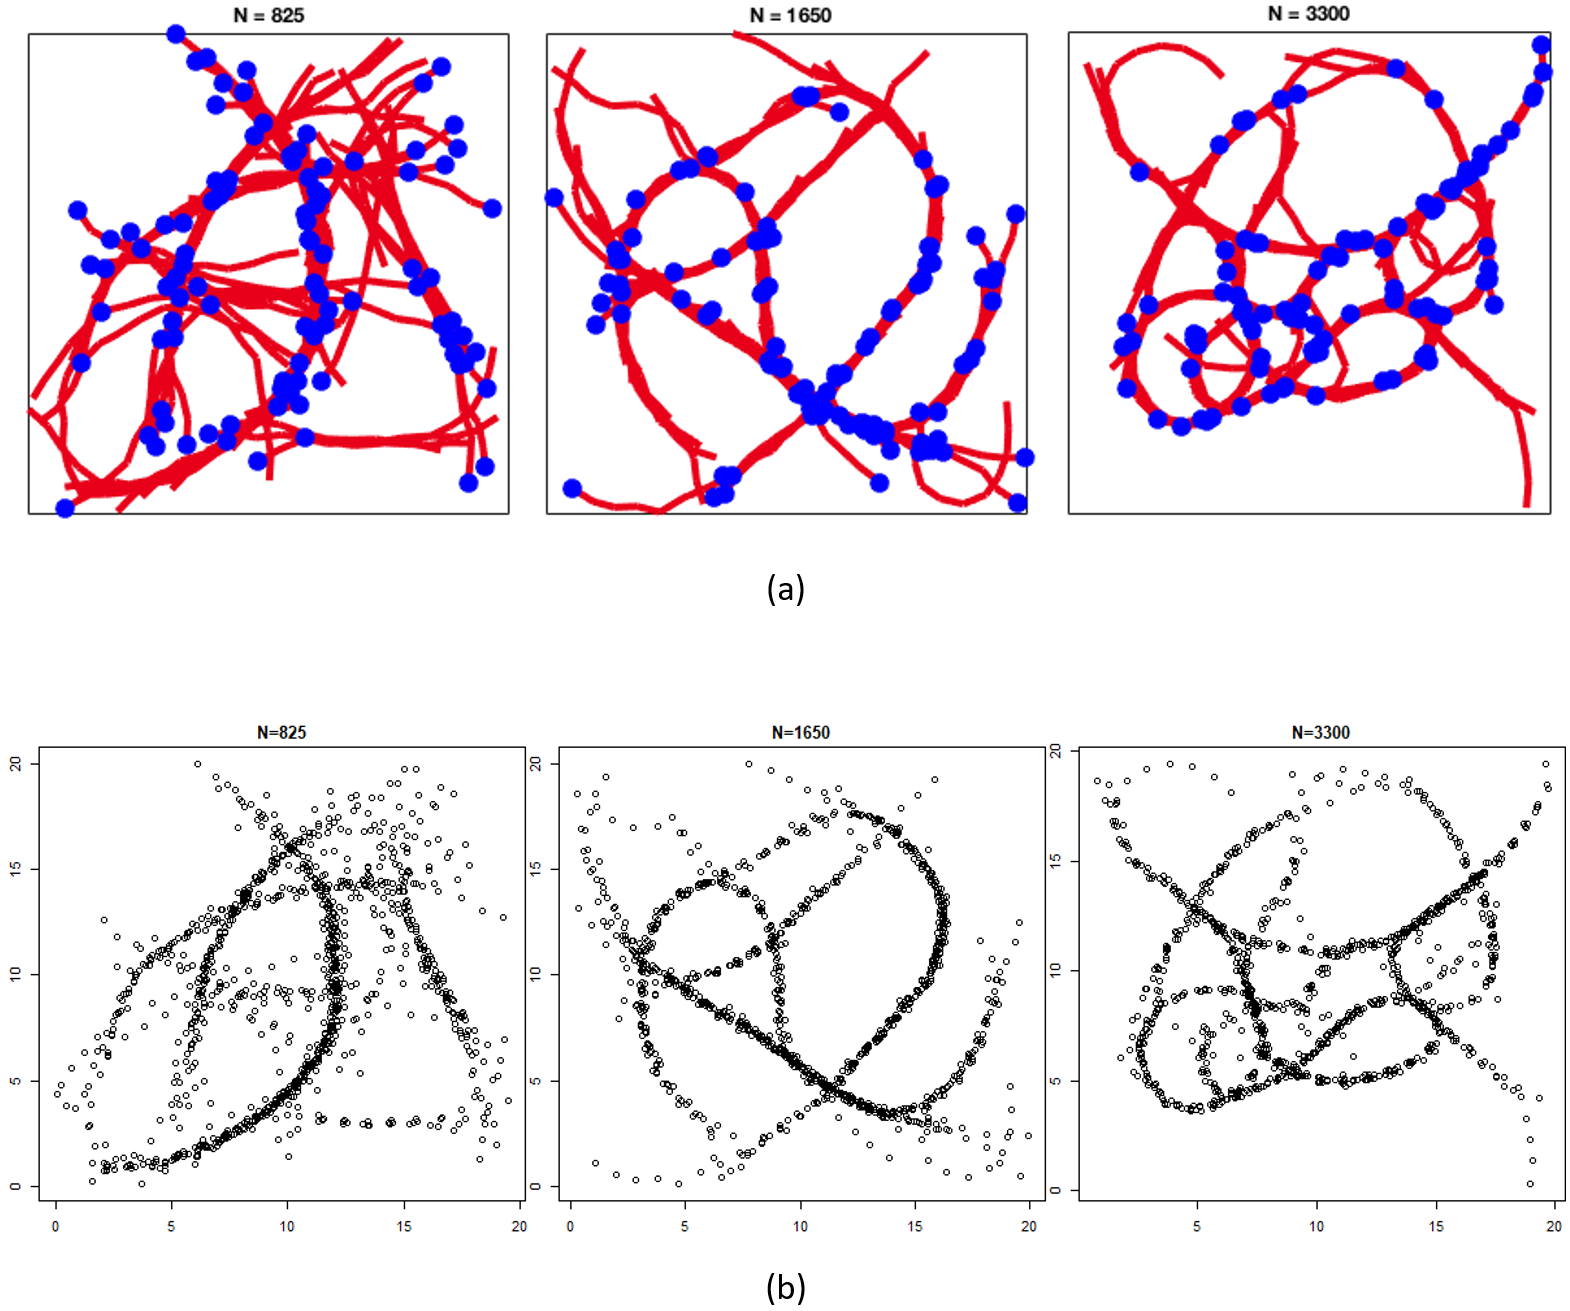
\includegraphics[width=1\textwidth]{rawdata.png}
	\end{center}
	\caption{Filament networks. Panel (a) shows three filament networks generated by $825$, $1650$ and $3300$ cross-linkers, respectively, in a $\SI{20}{\micro\metre} \times \SI{20}{\micro\metre}$ area. Each network contains $100$ filaments which are represented as red lines. The blue dots are the barbed ends of these filaments. Panel (b) shows the locations of the actin beads that make up the filaments exhibited in Panel (a).}
	\label{fig:rawdata}
\end{figure}


To classify filament networks, we need to build a structure which reveals geometric features hidden in the data. We construct this structure with simplicial complexes in the typical way of persistence homology by using the 2-dimensional coordinates of actin beads along the filaments as the initial nodes. Simplcial complexes provide a bridge between the data space and a topological space in which computation of distances between sets of data points can be realized. A simplicial complex is a finite collection of simplices of different dimensions such that faces of simplices are also simplices, and intersections of the simplices are either empty or a face of both \cite{edelsbrunner2010computational}. In particular, higher dimensional simplices are constructed from lower dimensional simplices. Vertices are 0-dim simplices. A 1-dim simplex is called an edge and is created by its two vertices as faces (note that a higher dimensional edge is constructed from lower dimensional points). A 2-dim simplex or a triangle has three edges as faces. Further more, a 3-dim simplex or a tetrahedron has four triangles as faces, another nesting of several lower dimensional features to build one of higher dimension.

%%%%%%%%%%%%%%%%%%%%%%%%%%%%%%%%%%%
In order to build simplicial complexes, we adopt the procedure of forming Vietoris-Rips complexes on each dataset (actin network) by introducing a sequence of $\epsilon$-balls with increasing radius $\epsilon$ centered at each data point (actin bead). Simplicial complexes are constructed based on intersections of these $\epsilon$-balls and each value of $\epsilon$ corresponds to an unordered group of homological features, which is called a homology group. Considering values of $\epsilon$ as a timeline, we only record when a homological feature appears and disappears. These indexes are called the birth times and death times of a particular homological feature. Moreover, the lifespan (death minus birth) of a homological feature is referred to as the feature's persistence. A set of homological features gives rise to a set of persistence measures. At the end of this procedure, when radius $\epsilon$ is sufficient larger so that the homology group remains unchanged even by further increase the radius, information of a filament network's persistence homology (the set of persistent homology measurements) is summarized in a persistence diagram.

To illustrate the process of building a persistence diagram, we provide a depiction of a simple network in Fig. \ref{fig:persistencediagram}. We show the data points in 2-dimensional space, investigating $\epsilon$ from $0$ to $1.25$ and recording 0-dim and 1-dim homological features. These features are interchangeably referred to as connected components and holes respectively. More exactly, 0-dim homological features measure the connectedness of the data and 1-dim homological features capture the number of one dimensional holes in the data. When $\epsilon$ is relatively small, five individual components are present. When $\epsilon$ increases to $0.71$, four $\epsilon$-balls in the upper half area have intersected and four components merge into one connected component. This simultaneously gives rise to a hole. When $\epsilon$ is enlarged to $0.85$, all components merge into one connected component, though the hole survives. When $\epsilon$ is continuously increases to $1$, the only 1-dim hole vanishes. No extra information is gained while $\epsilon$ is grown to $1.25$. The appearance and disappearance of 0-dim and 1-dim features are summarized as black dots (connect components) and red triangles (holes) in a persistence diagram at the end. Notice for $0$-dim homological features, $3$ connected components are born at $0$ and die at $0.71$, $1$ connected component is born at $0$ and dies at $1$, $1$ connected component is born at $0$ and survive to the end. For $1$-dim homological features, a $1$ hole is born at $0.71$ and dies at $1$. Thus, persistence homology provides information on the connectedness and holes induced from the Vietoris-Rips complexes on the points cloud. 

Overall, persistence homology indirectly summarizes the hidden shape of the data and transcribes this shape to the persistence diagram. With the persistent homology of each point cloud, a classifier can be generated either from the distance \cite{marchese2018signal} between persistence diagrams or by alternative vectorizations of the diagrams \cite{adams2017persistence,bubenik2015statistical,maroulas2018stable}.

\begin{figure}[!htbp]
	\begin{center}
		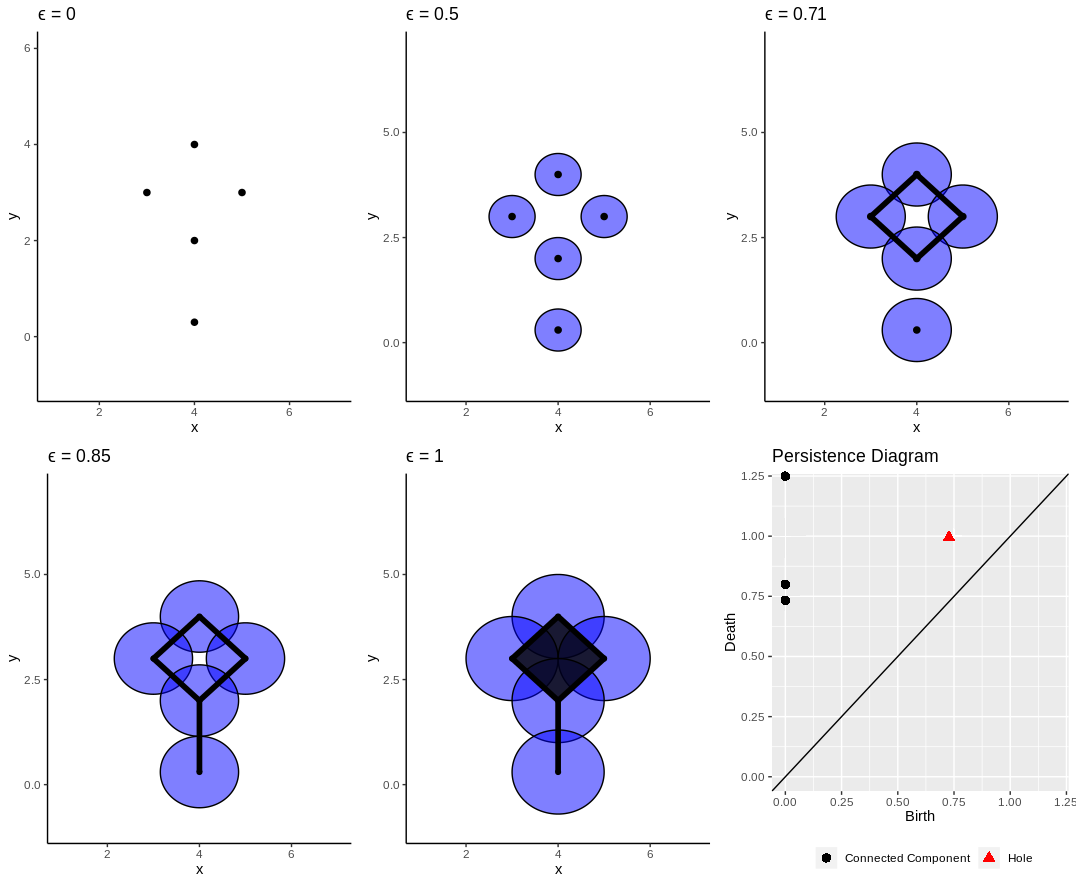
\includegraphics[width=1\textwidth]{pd_example.png}
	\end{center}
	\caption{Approach depiction of making persistence homology. Beginning from $\epsilon=0$, there are $5$ components. We show the key $\epsilon$ values where components are born or die. When $\epsilon=0.5$, $5$ components stay alive. When $\epsilon=0.71$, $4$ components connect into one connected component, forming a $1$ hole, thus $3$ components die and $1$ hole is born. When $\epsilon=0.85$, $2$ components further connect into $1$, therefore, $1$ more component dies. Finally, when $\epsilon=1$, the only $1$ hole dies and only the $1$ connected component survives. No additional homological change while $\epsilon$ is grown to $1.25$. The persistence homology of this complex is summarized in the persistence diagram.}
	\label{fig:persistencediagram}
\end{figure}

\section{Filament network classifier}
Once we have persistence diagrams corresponding to the point clouds of actin networks, we are ready to classify these networks. In this work, we propose two methodologies as candidates for a filament network classifier, one is distance-based method while the other one is based on a vectorization.

\subsection{Distance-based network classifier}
Given any two persistence diagrams, we need a way to quantify the difference between them in the space of persistence diagrams. In TDA, two methods are commonly used to calculate the distance between persistence diagrams: the Bottleneck and Wasserstein distances \cite{adams2017persistence,bubenik2015statistical,edelsbrunner2010computational,kerber2017geometry,wasserman2018topological}. These distances calculate the optimal (minimal) cost in matching the points between two persistence diagrams. They assume infinitely many points of infinite multiplicity on the diagonal (where birth equals death), so that off-carnality points are matched to a point in this artificial set. In addition to the Wasserstein and Bottleneck distances, in this work we adopt a new distance, called $d^c_p$ distance, which is proposed in \cite{marchese2018signal} and has been proved to be stable in \cite{maroulas2018stable}. The cardinality of a persistence diagram may carry important information in applications, especially for those homological features which die very quickly and may be considered as insignificant in Wasserstain distance. However, the $d^c_p$ distance accounts uneven cardinalities between persistence diagrams by assigning a regularization term with the parameter $c$ rather than connecting extra points to the diagonal as is done in the Wasserstein distance. This method allows one to adjust the weight assigned to data that might be considered "topological noise" to fit the particular use case.

\begin{definition}{1}
Let $D_X$ and $D_Y$ be two persistence diagrams with cardinalities $n$ and $m$ respectively such that $n \leq m$ and denote $D_x=\{ x_1,...,x_n \}$, $D_y=\{ y_1,...,y_m \}$. Let $c>0$ and $1\leq p <\infty$ be fixed parameters. The $d^c_p$ distance between two persistence diagrams $D_x$ and $D_y$ is
\begin{align}
    d^c_p(D_x,D_y)= \left( \frac{1}{m} \left( \min_{\pi \in \Pi_m} \sum^n_{l=1} min(c,||x_l-y_{\pi(l)}||_\infty)^p+c^P|m-n|  \right) \right)^{\frac{1}{p}},
    \label{eq:dpcdistance}
\end{align}
where $\Pi_m$ is the set of permutations of $(1,...,m)$. If $m<n$, define $d^c_p(D_x,D_y):=d^c_p(D_y,D_x)$.
\end{definition}

The $d^c_p$ distance not only calculates the distance of points in two persistence diagrams without the simulated points on the diagonal, it also adds a penalty term on the difference in cardinalities of the two sets of points. The parameter $c$ in eq. (\ref{eq:dpcdistance}) is a constant that controls the weight of penalization to be added in the $d^c_p$ distance. Larger values of $c$ will yield a larger penalization. The parameter $p$ is typically chosen as $2$ since this corresponds to the Euclidean distance. We tend to evaluate $c$ between $0$ and $1$ as these have been empirically found to be appropriate options in real-world applications \cite{maroulas2018stable}.

Since persistence diagrams can summarize the homological features of multiple dimensions in one diagram, such as in the last panel of Fig. \ref{fig:persistencediagram}, the persistence diagram contains both $0$-dim features(connected components) with cardinality $5$ and $1$-dim features(holes) with cardinality $1$. We can further define the $d^c_p$ distance of a certain dimensional feature between a persistence diagram and a group of persistence diagrams.

\begin{definition}{2}
Denote $\D$ as a collection of persistence diagrams in the same class. For a specific $\beta$-dim homological feature, $\beta=0,1,2,...$, the $d^c_p$ distance between a persistence diagram $D_x$ and the set of persistence diagrams $\D$ is
\begin{align}
    d_\beta (D_x,\D)=\frac{1}{|\D|}\sum_{D \in \D} d^c_p(D_x,D),
    \label{dpcsets}
\end{align}
where $|\D|$ represents the size of class $\D$.
\end{definition}

With all preparations above complete, we can build the $d^c_p$-based network classifier. For $K$ classes of filament networks, every network in a class is generated under a unique set of constraints. Therefore, we have $K$ sets of persistence diagrams, where each set corresponds to a class of network generated under unique constraints. Given a new filament network with its persistence diagram $D'$, our goal is to classify under which constraints the network was most likely generated, i.e. to which class $k$ it most likely belongs. We can estimate this membership by calculating the distance between $D'$ and each class of persistence diagrams. We then assign the new network to the class with the smallest distance. Additionally, we parameterize the relative weights for different dimensions of homological features in the calculation of the distance and force the weights' sum to $1$. The classifier is summarized in Algorithm \ref{alg:dpcclassifier}.

\begin{algorithm}[!htbp]
	Let $B$ is highest dimension of homological features under consideration.\\ 1. Take the training set $T_1, T_2,..., T_K$ from each class of diagrams $\D_1,\D_2,...,\D_K$, \\
	2. For a new network with its corresponding persistence diagram $D'$, compute
	\begin{align}
	    d(D',T_k)=\sum^B_{\beta=0} w_\beta d_\beta (D',T_k),
	\end{align}
	\ \ \  where $\sum^B_{\beta=0}w_\beta=1$, and $w_\beta$ determine how much $\beta$-dim homological feature is considered,\\
	3. Assign $D'$ a class label $c'$ such that,
	\begin{align}
	    c'=\argminA_{1\leq k \leq K} d(D',T_k),
	\end{align}
	\caption{$d^c_p$-based network classifier}
	\label{alg:dpcclassifier}
\end{algorithm}

\subsection{Non-distance-based network classifier}

\subsubsection{Sub-sampling approach}

In a second analytical branch, rather than work on the coordinates of the actin beads directly, we took several pre-processing steps in order to extract more information from the provided network samples. The actin bead data included both spatial coordinates as well as an index indicating the filament sampled. That is, for our networks $\{X_1, X_2... X_{150}\}$, we had 100 filaments in each network $\{F_1, F_2... F_{100}\}$ and therefor our sampled points have features $x, y$, and $f$, where  $x$ and $y$ are the coordinates in the plane and $f$ is the index in the identity map of $F$. 

Using R’s spatial package, each filament was constructed by connecting the ($x$,$y$) bead-coordinates in each filament. A single filament network was then constructed as a multiline object from the corresponding collection of lines formed from the bead-coordinates. These multiline objects were then projected onto square grids of $200\times200$ cells. Then, for each network we sampled the multiline object into a grid with the identity function (i.e. the grid cells have value 0 unless a line and grid cell intersect then the value of the grid cell goes to 1). We now had a grid of 4000 cell values taking $\{0,1\}$. We filtered these 4000 values to only those of value 1 and used the corresponding planar coordinates to build our new simplicial complexes and persistence diagrams. All re-sampling steps are summarized in Algorithm \ref{alg:resample}. 

\begin{algorithm}[!htbp]
	Let $X_i \in \{X_1...X_{150}\}$ the set of simulated actin networks. \\
    Let $a \in \{A_{i,(x,y,f)}...A_{i,(x,y,f)}\}$ the set of points in $X_i$. $a$ is a pair, $(i, (x,y,f))$, where $i$ is an index to $X_i$, $x$ and $y$ are planar coordinates and $f$ is an index to a filament of $X_i$, $F_{i,f} \in \{F_{i,1}...F_{i,100}\}$, along which $a$ lies. See Panel A of Fig. \ref{fig:resample_algorithm} for a graphical depiction of one $X_i$. For simplicity, we will describe how our algorithm is applied to $X_1$:\\\\
	1. Reconstruct the paths of each $F_{1,f}$ by connecting $A_{1,(x,y,f)}$. See Panel B, Fig. \ref{fig:resample_algorithm}.\\
	2. We project $F_1$ onto a 200x200 square lattice with the same bounds as the given by the data. The cells, $c_{x,y}$ of the lattice take values $\{0,1\}$, where $c_{x,y}=1$ if it is intersected by one of $F_1$ and 0 otherwise. See Panel C of Fig. \ref{fig:resample_algorithm}.\\
	3. Retain only $c_{x,y}$ where $c_{x,y}=1$.\\
	4. Draw 1000 random $c_{x,y}$ without replacement and call these the elements of $R_{1, r}$. Repeat this twice so that $r$ indexes three new samples drawn from $X_1$. The three colors in Panel D of Fig. \ref{fig:resample_algorithm} denote the index $r$.\\
	5. Generate three separate persistence diagrams, $D_{1,r}$, for the new samples $R_{1,r}$. Shown in Panel E of Fig. \ref{fig:resample_algorithm}.
	\caption{Re-sampling Algorithm}
	\label{alg:resample}
\end{algorithm}

Due to the exponential growth of the computation of the Vietoris-Rips complex, rather than computing a Vietoris-Rips complex per network, $1000$ points were randomly sampled from each network $3$ times without replacement. This gives us $3$ sets of $1000$ points per network. This increased the sample size from $150$ to $450$ networks. We computed persistence diagrams for these $450$ networks and could used these to construct a classifier using the same procedure as outlined in Algorithm \ref{alg:dpcclassifier}.

\begin{figure}[tbp]
	\begin{center}
		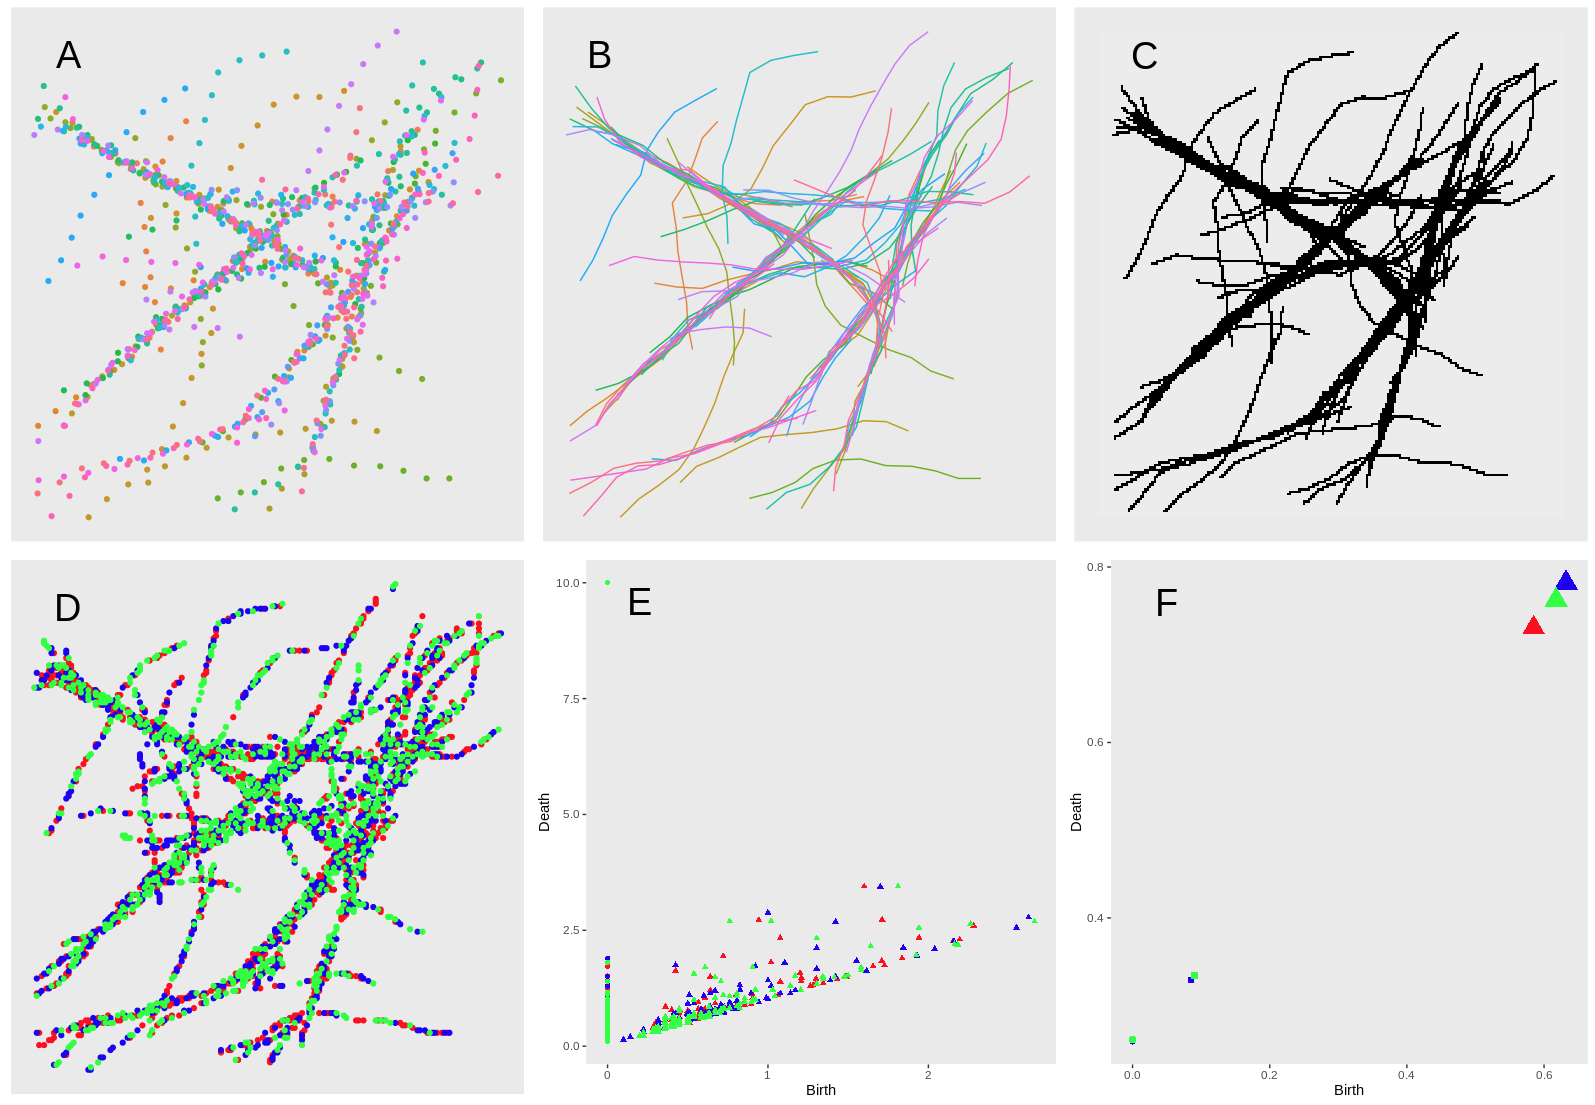
\includegraphics[width=1\textwidth]{resample_algo.PNG}
	\end{center}
	\caption{Example of one filament construction (B) from the supplied point cloud (A), rasterization (C), re-sampling (D), construction of persistence diagram (E) and vectorization of persistence diagram (F). The point cloud in (A) was supplied with an index that allowed for the constrution of the filaments in (B); note the coloring. This was projected onto a 200x200 raster (C). The raster was sampled into 3 sets (colored) of 1000 points (D) without replacement and the x,y coordinates are used to generate a VR complex. The persistence diagrams and vectorizations in (E) and (F) are colored the same as (D), to show the variability that arises in the vectorized persistence diagram features when this approach is taken.}
	\label{fig:resample_algorithm}
\end{figure}


\subsubsection{Persistence vectorization/classification}

In addition to distance based classification, a classification was performed on vectorized features of the persistence diagrams. A matrix was generated from the persistence diagrams which had row entries for each diagram and column features with the mean and standard error of persistence diagrams considering only the $0^{th}$ or $1^{th}$ persistence features alone and all topological features. That is, for each filament network, there is one persistence diagram which corresponds to one row of the vectorized matrix with mean and standard error of birth or death times for $0^{th}$, $1^{th}$, or all features. This gives us 12 columnar features. However, the mean and standard error of births for $0^{th}$ features are constant 0 and are not considered. Therefor, we are left with 10 entries per vector. The vectorization procedure is shown in Algorithm \ref{alg:vectorization}. 

\begin{algorithm}[!htbp]
	We vectorize $D_{1,r}$ from Algorithm 2 by taking the mean $birth$ and mean $death$ of connected components and holes. These data are plotted in Panel F of Figure 3. For $D_{1,r}$ we have 3 row-vectors in the form:
	\begin{center}
	    $v_{1,r}$ =
        $\begin{bmatrix}
            \bar{x}(\mathrm{Death~of~Connected~components})\\
            s(\mathrm{Death~of~Connected~components})\\
            \bar{x}(\mathrm{Birth~of~holes})\\
            s(\mathrm{Birth~of~holes})\\
            \bar{x}(\mathrm{Death~of~holes})\\
            s(\mathrm{Death~of~holes})\\
            \bar{x}(\mathrm{Birth~of~all~features})\\
            s(\mathrm{Birth~of~all~features})\\
            \bar{x}(\mathrm{Death~of~all~features})\\
            s(\mathrm{Death~of~all~features})\\
        \end{bmatrix}$
    \end{center}
	Note: the mean $\bar{x}$ and standard error $s$ of the birth of connected components would be $0$ for all vectors, so these are not found in $v_{1,r}$. Repeat for all $X_i$. Our complete matrix of data has a final dimension $450\times10$.\\
	\caption{Vectorization of persistence diagrams}
	\label{alg:vectorization}
\end{algorithm}

\section{Classification result}

\subsection{$d^c_p$-based classifier}
In our data set, we are provided three classes of filament networks. Each class of filament network is generated with a different number of cross-linking proteins. Each class contains $50$ samples. Therefore, there are total of $150$ individual provided filament networks. 

In order to compare classifiers, we employed $10$-fold cross validation to estimate overall classification accuracy. All of the networks are randomly partitioned into $10$ mutually exclusive sets. $9$ partitions are selected as a training set, while the remaining $1$ partition is used for testing. We repeat the classification $10$ times such that every partition acts as a testing set exactly once. We consider the overall classification accuracy rate as the mean accuracy across all partitions.

After generating the persistence diagram for each filament network from the locations of actin beads, we tested our classifier on this data set using the $d^c_p$-based classifier in Algorithm~\ref{alg:dpcclassifier}. We consider only $0$-dim and $1$-dim topological homological features. We chose $p=2$ to imitate Euclidean distance. The choices of parameter $w_0, w_1, c$ were found to be optimal based on cross validation. When $w_0=0.5, w_1=0.5$, connected components and holes are weighted equally, and $c=0.2$ gives a relatively small contribution from the cardinality difference in the $d^c_p$ distances, the best classification accuracy rate is $89\%$.

\subsection{non-distence based}

A support vector machine (SVM) was used to develop a network classifier based on the 3-times re-sampled and vectorized persistence diagrams. $10$-fold cross-validation was again used to assess the accuracy of the SVM classifier. Accuracy was measured only on one of the three sub-sampled networks $R_{i,1}$ per filament network $X_i$ so as to fairly compare to the methods without re-sampling. The mean accuracy of the classifier was 96.3\%. This was the highest accuracy attained on this set of simulated networks.

\subsection{Comparison to other classifiers}
We also list the accuracy rate by using other classifier in Table \ref{tab:accuracyrate}.
\begin{table}[!htb]
	\begin{center}
		\begin{tabular}{c|c}
			\hline
			\textbf{classifier} & \textbf{accuracy} \\
			\hline
			SVM, re-sampled & 96\%  \\
			\hline
			$d^c_p$-based & 89\%  \\
			\hline
			Wasserstein-based, re-sampled & 87\%  \\
			\hline
			Wasserstein-based & 83\%  \\
			\hline
			Bayes Factor \cite{maroulas2019bayesian} & 83\%  \\
			\hline
			SVM PI \cite{adams2017persistence} & 75\%  \\
			\hline
			Neural Net PI & 71\%  \\
			\hline
			SVM Raster & 65\%  \\
			\hline
			Random Forest Raster & 55\%  \\
			\hline
		\end{tabular}
		\caption{Accuracy rate of classifiers}\label{tab:accuracyrate}
	\end{center}
\end{table}

Our findings show that re-sampling of data can produce a more reliable filament network classifier even when data are mapped to a topological space and summarized in persistence diagrams. The $d^c_p$-based classifier performed much better than Wasserstein-based classifier. Our re-sampled and vectorized persistence diagram based classifier and $d^c_p$-based classifier are superior than any other common classifiers. These findings suggest that future with with real data microscopy data may be classified with similar methods.

\subsection{Application to classifying myosin mutants}
We are given labeled images of cells belonging to one of two classes: myosin mutant (MM) or wild type (WT). The MM cells have a genetic knockout such that they do not a produce one of their myosin proteins. The WT cells are the control with no knockout. Myosin motor proteins are known, via empirical observation, to influence the connectivity and shape of the actin filament network. This experiment differs from our synthetic experiment in that our synthetic experiment involved the direct manipulation of the actin network through changes in cross-linker abundance. Whereas cross-linking is fundamental to the structure of the actin network, the linkage betweeen mysoin motors and actin networks is more complex and likely modulated by several interacting factors.

\begin{figure}[H]
	\begin{center}
		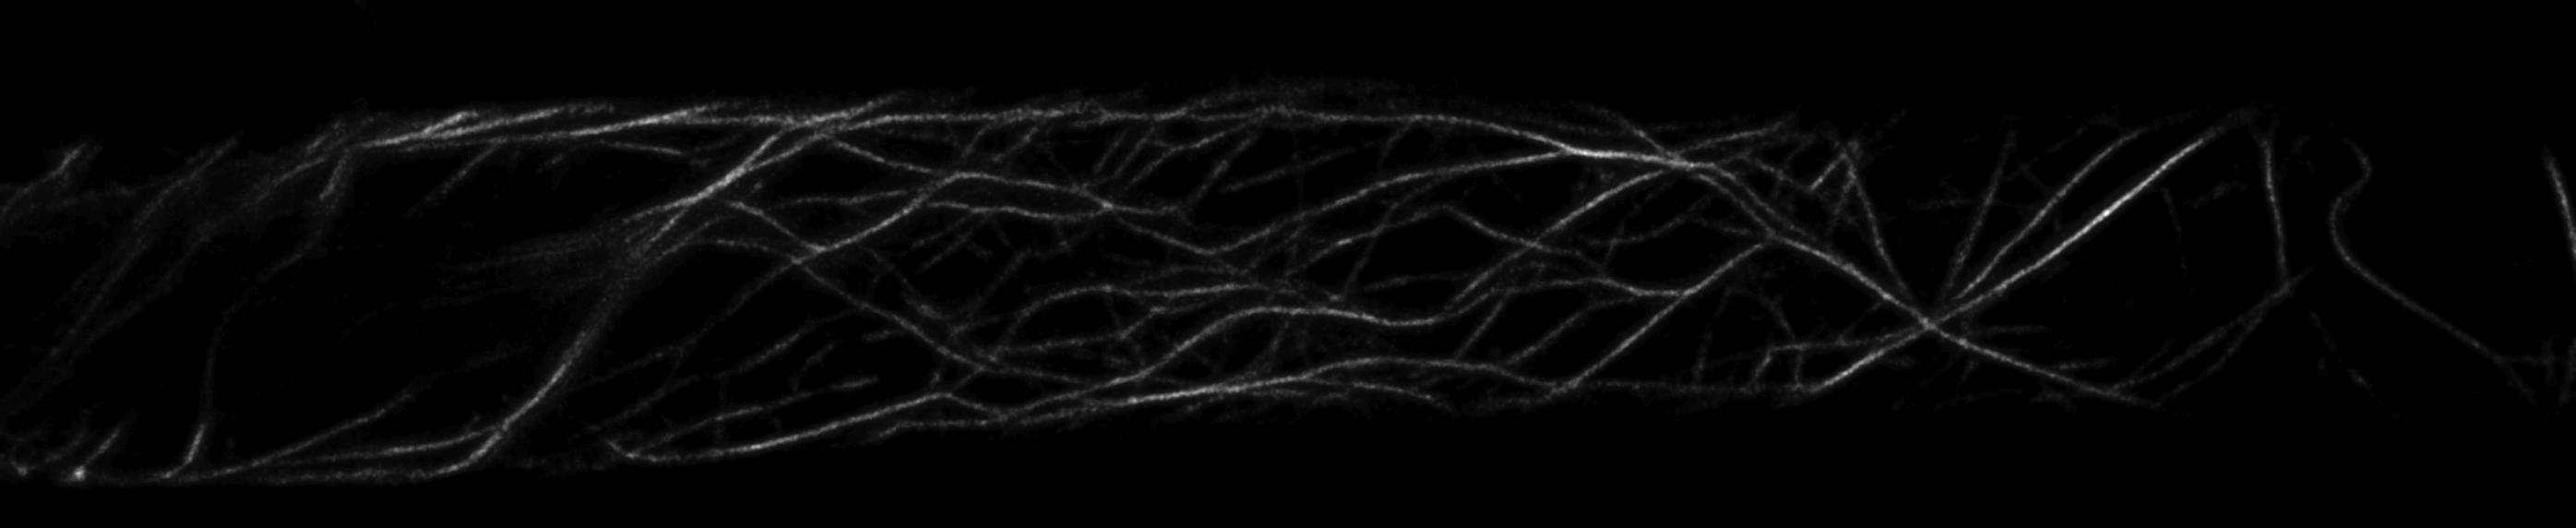
\includegraphics[width=.9\textwidth]{../../fig/wtCell.png}
	\end{center}
	\caption{Example of a raw WT cell image.}
	\label{fig:wtCell}
\end{figure}

We perform classification of MMs and WTs using our top classifier, the re-sampled SVM. The data are provided as tifs from 22 MM and 20 WT cells. Each tif is a a very high resolution (roughly 2500x500 pixels with 0.043 $\mathrm{\mu m}^2$ pixels) grayscale image, wherein the pixel values are an 8-bit inensity. We perform preprocessing on the images simply by performing a gaussian blur and then thresholding to the top $\frac{1}{3}$ of values. The thresholded image is then a grid of values taking only 0 or 1, where 1 indicates the presense of a filament. We then take the processed images and proceed in classification from step (C) in Figure \ref{fig:resample_algorithm}, resampling, computing PDs, vecorizing the PDs, and finally classifying with an SVM. We find a cross-validated (k=5) accuracy of roughly 73\%.

Interpretation of these results is complicated by our uncertainty of the true, cumulative impact of the moyin knockout on the actin network. While the accuracy in this experiment is significantly lower than found in the analysis of the synthetic data, this could easily be explained by the single motor protein knockout having a relatively minor impact on actin organization when compared with up or down regualtion of cross-linkers. Out of curiosity, we conducted a small survey (\textit{n}=6), wherein we asked respondents who were familiar with the experiment to sepparate the cells into two classes. We found that respondents had an average accuracy of 63\%, with a minimum accuracy of random chance and a maximum accuracy of 75\%. Since our algorithm is (on average) more effective than manual classification by an expert, we conclude that there is likely a weak relationship between this mysoin knockout and actin network structure, and our classification algorithm is likely running into the ceiling of discernible difference in classes.


\section{Conclusion}
In this work, we successfully classified simulated actin filament networks generated under different initial conditions with very high accuracy. We combined a machine learning framework with TDA and proposed two classifiers. One is a distance-based classifier based on a new advanced distance on the persistence diagram space, i.e., the $d^c_p$ distance; Another one is a non-distance-based classifier with re-sampling and persistence vectorization. Both of these methods were built on the foundation of topological homology by encoding geometric features hidden in the data into the topological features and summarizing those into persistence diagrams.

From these results, we are able to confidently classify actin filament networks based on unique inital conditions. Accordingly, these methods could reveal the key factors in the filament network generating process and provide biologists with the opportunities to uncover the interaction of motor proteins, actin networks and streaming. In addition, we show that it is possible to classify cells by images of their actin networks, since our data reflects a 2 dimensional projection of the network such as would come from microscopy. Overall, our work is the first time that actin filament networks have been studied by topological classification, researchers could further advance their understanding of cell physiology through this work and future research. 

\clearpage	
%\nocite{*}
\bibliographystyle{plain}
\bibliography{bibliography}


\end{document}
